
\section{引言}
稍微了解Chromium应用的人都会清楚Chromium为多进程应用。
关于其进程模型的框架在其官方文档的多进程框架(\url{https://www.chromium.org/developers/design-documents/multi-process-architecture})一节有详细的介绍。
本文不是官方文档的翻译,所以不会设计太多理论性的介绍,如果想要了解更多理论知识,可以查看官方文档的相关章节或浏览技术论坛。
本文的重点在于研究Chromium各进程的启动流程、以及进程的启动策略,重点在于具体实现和具体流程的分析。

本文会按照Browser进程、Render进程、GPU进程和Plugein进程的顺序进行研究,其他分类的进程会在这四类进程研究过程中进行分析。
Chromium也包含多个平台的实现,目前本文主要研究Windows平台和Linux平台,其他平台暂时不做研究。
Chromium可以编译为多个形式的应用,本文主要以比较简单的content\_shell作为研究对象。

\section{Chromium多进程模型简介}

\begin{figure}[H] 
  \centering 
  \includegraphics[width=0.80\textwidth]{image/process_study/multi_process_architecture.png} 
  \caption{chromium多进程模型示意图} \label{fig:multi_process_architecture} 
\end{figure}

如图~\ref{fig:multi_process_architecture}所示,是chromium官方文档给出的多进程模型的简单示意图。
图中主要描绘了Browser进程和Render进程的关系。
其中,最上面的那个方框代表Browser主进程,是UI线程所在的进程,负责与用户交互、处理网络请求和管理Render进程等。
从图中可以看出,Render进程可以不止一个,它主要任务是渲染打开的网页。
但是并不能简单的理解为一个网页就是一个Rander进程,这个关系是可以通过启动参数配置的,后续会详细讨论这个问题。

可以从图中看出,Browser进程是通过RenderProcessHost和RenderProcess对象管理Render进程的。
RenderProcessHost对象与Render进程中的RenderProcess对象一一对应。
每一个Render进程都有且只有一个全局的RenderProcess对象,Render进程可以通过它和Browser进程通信。

每个Render进程都会有一个或多个RenderView对象,它们受RenderProcess对象管理,代表一个使用Blink引擎渲染的区域。
同样,在Browser进程中的RenderProcessHost对象管理着与RenderView对应的RenderViewHost对象。
在chromium中,还存在RenderWidgetHost和RenderWidget类,作为RenderViewHost和RenderView父类。
RenderProcess、RenderWidge、RenderView对Browser和Render进程之间的消息传递具有重要的作用,后续的章节会作出详细的研究。

在Chromium启动之初,最先启动的是Browser进程,由它来启动其他进程。
研究的四类进程中Browser进程和GPU进程都只会有一个,而Render进程和插件进程可以存在多个。
另外,Chromium提供了启动参数(--single-process)可以设置为单进程模式,就是所有的功能运行在一个进程中。

\section{Browser进程启动流程}
Browser作为Chromium系统的主进程,最先启动,其启动的流程自然从main函数开始的(事实上,随着我们的研究,会了解到所有进程的启动都是从main函数开始)。
main函数看起来非常的简洁,对于content\_shell它定义在shell\_main.cc文件中,其代码如下:

\begin{spacing}{1.0}
\begin{lstlisting}[language={C++}]
int main(int argc, const char** argv) {
#if defined(OS_MACOSX)
  // Do the delegate work in shell_content_main to avoid having to export the
  // delegate types.
  return ::ContentMain(argc, argv);
#else
  content::ShellMainDelegate delegate;
  content::ContentMainParams params(&delegate);
  params.argc = argc;
  params.argv = argv;
  return content::ContentMain(params);
#endif  // OS_MACOSX
}
\end{lstlisting}
\end{spacing}

在这段代码中定义了两个对象,它们的类型是ShellMainDelegate与ContentMainParams,最后调用了ContentMain函数。
ContentMain函数也是非常简单的:

\begin{spacing}{1.0}
\begin{lstlisting}[language={C++}]
int ContentMain(const ContentMainParams& params) {
  std::unique_ptr<ContentMainRunner> main_runner(ContentMainRunner::Create());

  int exit_code = main_runner->Initialize(params);
  if (exit_code >= 0)
    return exit_code;

  exit_code = main_runner->Run();

  main_runner->Shutdown();

  return exit_code;
}
\end{lstlisting}
\end{spacing}

从以上的代码可以看出,Browser进程启动之初,最终是执行了ContentMainRunner接口的Run方法。
其实,不止Browser进程,其他进程也会执行同样的流程,那么就让我们分析一下这些类以及后续的调用流程吧。

\begin{figure}[H] 
  \centering 
  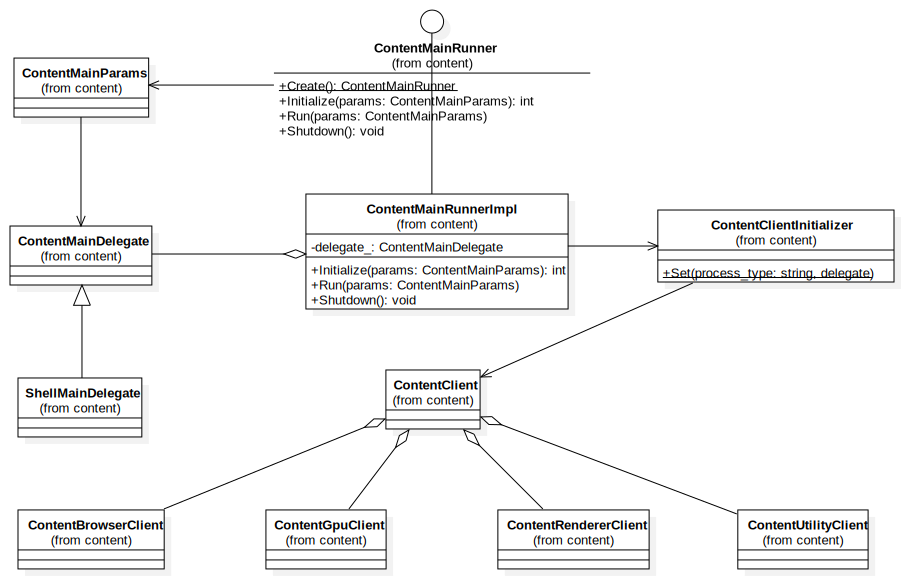
\includegraphics[width=0.90\textwidth]{image/process_study/ContentMainRunner.pdf} 
  \caption{ContentMainRunner相关类图} \label{fig:ContentMainRunnerClass} 
\end{figure}

如图~\ref{fig:ContentMainRunnerClass}所示,ContentMainRunnerImpl是ContentMainRunner接口的实现类,
也是这个过程中主要的工作对象,其生命周期与Browser进程的生命周期相同。
在ContentMainRunnerImpl类中主要有两个成员变量需要注意:

一个为ContentMainDelegate类型的delegate\_
变量,在content\_shell应用中,其实际为ShellMainDelegate对象。
在shell\_main.cc文件中的mian函数中创建,通过ContentMainParams变量传入ContentMainRunnerImpl变量中。
其主要负责在进程启动过程以及后续的一些节点上作出一些配置,如在进程刚刚启动时初始化LOG模块,添加一些调试信息等。
另外,它也负责设置ContentClient变量。

另一个变量就是ContentClient变量了,ContentMainRunnerImpl类中定义一个成员变量empty\_content\_client\_。
其主要作用是作为默认的ContentClient变量,在ShellMainDelegate中定义了一些ContentClient变量,会在BasicStartupComplete
方法中设置为进程的ContentClient变量,如果没有设置,就会使用empty\_content\_client\_。
ContentClient变量是通过content::GetContentClient方法获取的,其为全局变量。
通过ContentClient变量又可以获取到对应进程的Client,如ContentBrowserClient、ContentGpuClient、ContentRendererClient等。
这些Client类在Chromium的不同编译中有着不同的实现,它们是维护浏览器的重要接口类。
它们定义的一些接口和回调可以影响浏览器的内部逻辑,如:CanCommitURL可以阻止一些不想要的请求;AllowGetCookie、AllowSetCookie
可以控制访问网站对Cookie操作;AllowCertificateError可以处理当发生证书错误时的具体行为等等。

在content\_shell应用中,delegate\_变量和ContentClient变量分别对应ShellMainDelegate对象和ShellContentClient对象。
ShellContentClient对象中保存的Client类是ShellContentBrowserClient和ShellContentRendererClient等。
为了修改浏览器的一些逻辑,肯定会对这些类作出改动,我认为最好的方法是继承这些类,而不是对它直接修改。

\begin{figure}[H] 
  \centering 
  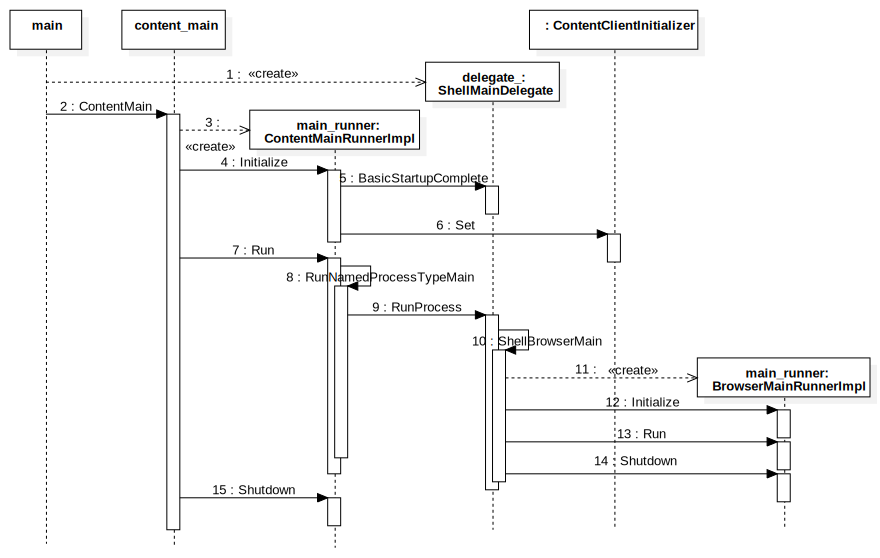
\includegraphics[width=0.90\textwidth]{image/process_study/ContentMainRunnerSequence.pdf} 
  \caption{Bowser进程启动初始流程} \label{fig:ContentMainRunnerSequence} 
\end{figure}

如图~\ref{fig:ContentMainRunnerSequence},是浏览器进程从开始启动,到真正按进程类型去执行相关的功能的时序图。其中:
\begin{itemize}
  \item 在ContentMainRunnerImpl类的Initialize方法中进行进程的启动准备工作,对于所以进程都是执行同一个方法。
  所以,这个方法非常复杂。在这个方法中会去调用delegate\_对象的BasicStartupComplete方法,进而会重新设置ContentClient对象。
  另外,命令行对象的初始化也在这里进程。
  \item 随着ContentMainRunnerImpl类的Run方法的调用,进程开始运转。
  Run方法是阻塞的,它会一直持续到整个进程结束,其最后是启动一个MessageLoop这点会在介绍消息队列的章节详细介绍。
  在Run发放中会调用RunNamedProcessTypeMain方法,用来根据不同进程类型执行不同代码的逻辑。
  具体到Browser进程,会执行BrowserMain方法,还有其他诸如RendererMain、RendererMain、UtilityMain、RunZygote等方法,
  会在其对应的具体进程中详细讨论。
  也就是说,在调用BrowserMain方法之前,所有的进程的逻辑都是相同的,
  Browser进程启动过程与其他进程相比产生分歧也是从BrowserMain方法开始。
\end{itemize}

\subsection{Browser进程主线程启动流程}


BrowserMainRunner
BrowserMainRunnerImpl

BrowserMainLoop
ShellBrowserMainParts

浏览器Browser进程启动后,直接运行UI线程,UI线程又创建其他6个线程
在BrowserMainLoop::CreateThreads函数中创建浏览器其他线程


\section{Render进程启动流程}

为什么设置的log在render进程中失效

\section{Render进程的启动策略}

\section{Browser进程和Render进程重要类的对应关系}
